\section{Storia della lavatrice}
Tra tutti gli elettrodomestici moderni, la lavatrice è quello che ha maggiormente cambiato il modo di vita di tutti i giorni, dal momento che prima della sua diffusione il lavaggio di indumenti assorbiva una grande quantità di tempo ed energia. Infatti, si trattava di una tecnica puramente manuale e piuttosto rudimentale, basata sull’utilizzo dell’acqua corrente e con impiego di sostanze naturali volte alla rimozione dello sporco (sabbia, grasso naturale) \cite{de2002industrie}.


I primi prototipi di lavatrice arrivarono a metà del ‘700 proponendo di fatto una meccanizzazione del processo, attraverso lo sfregamento ripetuto dei panni e determinandone però una notevole usura.
A Napoli, nel 1851 si riportano l’impiego di macchine ad energia idraulica per la pulizia di panni attraverso una soluzione alcalina e simulando meccanicamente il movimento manuale 
\cite{de2002industrie}.


La vera rivoluzione arrivò con un dispositivo sviluppato in America da un mercante di nome William Blackstone. Si trattava di un barile di legno (Figura \ref{Figura 1}), riempito di acqua calda e sapone all’interno del quale i panni erano scossi da un asse dotato di lunghi pioli, che si muoveva manualmente in alto e in basso: chiamato agitatore. Il vantaggio consisteva nel forzare il detergente all’interno delle fibre sporche dei tessuti.


\begin{figure}[h!]
    \centering
    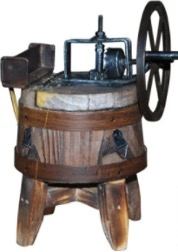
\includegraphics[scale=0.4]{Immagini/Senza titolo.jpg}
    \caption{Prototipo sviluppato da William Blackstone.}
    \label{Figura 1}
\end{figure}

Negli anni ’20 ci fu anche la sperimentazione di tecniche nuove come l’introduzione delle lavatrici a cestello ad asse orizzontale, non in grado di garantire però un risultato elevato in termini qualitativi e per questo impiegate soprattutto in ambito industriale \cite{asquer2007rivoluzione}.

Con il termine del secondo conflitto mondiale, soprattutto in Europa venne a nascere un’esigenza di benessere e nuove esigenze che permisero, insieme allo slancio economico, lo sviluppo e la diffusione delle lavatrici anche a livello domestico. 
In Italia negli anni ’60 si adottò inizialmente per una macchina avente un agitatore ed una seconda vasca per la strizzatura, modello americano (Figura \ref{fig:my_label}), per poi importare numerosi modelli dalla Germania basati però sul cestello ad asse orizzontale e migliorandoli ulteriormente dal punto di vista tecnologico \cite{asquer2007rivoluzione}.

\begin{figure}[H]
    \centering
    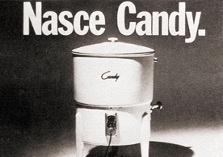
\includegraphics{Immagini/candy.jpg}
    \caption{Candy modello 50.}
    \label{fig:my_label}
\end{figure}
